\documentclass[12pt, a4paper]{article}
\usepackage[utf8]{inputenc}
\usepackage[default,scale=0.95]{opensans}
\usepackage[labelfont=bf]{caption}


\usepackage{fancyhdr}
\usepackage{url}
\usepackage{hyperref}

\usepackage{fancyvrb}
\usepackage{hyperref}
\usepackage{pgf}
\usepackage{float}
\usepackage{subcaption}
\usepackage{graphicx}



\hypersetup{
    colorlinks=true,
    linkcolor=blue,
    filecolor=magenta,
    urlcolor=cyan,
}


\def\myname{Sam Shahriari}
\def\assignment{Assignment 3}
\def\course{DD2424}



\author{Sam Shahriari}
\title{\course: \assignment}

\pagestyle{fancy}
\fancyhf{}
\rhead{\myname}
\chead{\assignment}
\lhead{\course}
\cfoot{ - \thepage \ -}
\renewcommand{\headrulewidth}{.1pt}


\begin{document}
\maketitle
\section{Gradient}
To check that my analytical calculation of the gradient was correct, I compared it to a numerical estimation for the same points and features. The numerical estimation was calculated by the given function\texttt{ComputeGrads\-NumSlow()} which uses centered difference formula. It was tested on different batch sizes and lambdas and also with and without batch normalization. None of the absolute or relative errors were above $10^{-6}$ and therefore I draw the conclusion that my implementation is correct.
More detailed results of the testing can be found in \autoref{gradientData}.
\section{3-layer network}
Two 3-layer networks, with 50 nodes per layer, were trained with cyclical learning rate on training set consisting of 45000 images and validation set of 5000 images. The following hyperparameters were used: $\eta_{min} = 10^{-5}, \eta_{max} = 10^{-1}, \lambda=0.005, n_s = 2250 $ and $n_{batch}=100$. The weights were He-initialized. After two training cycles the accuracies on the test data for batch normalization was $53.53\%$ and without batch normalization the accuracy was $52.97\%$. As the difference in accuracy is small for the 3-layer network it does not seem that batch normalization improves the results in a significant way.

\begin{figure}[H]
    \centering
    \begin{subfigure}{0.45\textwidth}
        \centering
        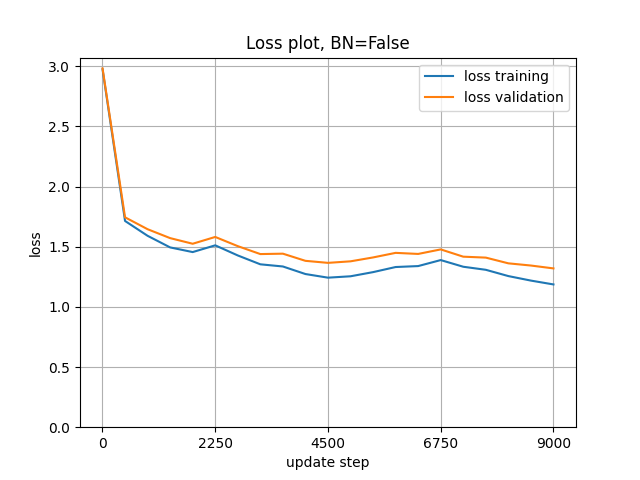
\includegraphics[width=\textwidth]{results/2-2250-3-loss-False.png}
    \end{subfigure}
    \hfill
    \begin{subfigure}{0.45\textwidth}
        \centering
        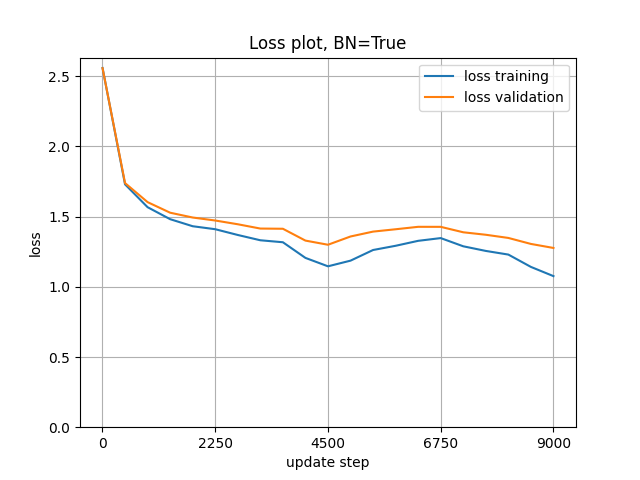
\includegraphics[width=\textwidth]{results/2-2250-3-loss-True.png}
    \end{subfigure}
    \caption{Loss plots for 3-layer networks}
    \label{fig:3-layer}
\end{figure}
\section{9-layer network}
For the 9-layer networks the following number of hidden nodes were used per layer; 50, 30, 20, 20, 10, 10, 10, 10. The other hyperparameters was the same as for the 3-layer networks. Here it was clear that batch normalization greatly improved the results,  $52.27\%$ accuracy compared to $41.75\%$.


\begin{figure}[H]
    \centering
    \begin{subfigure}{0.45\textwidth}
        \centering
        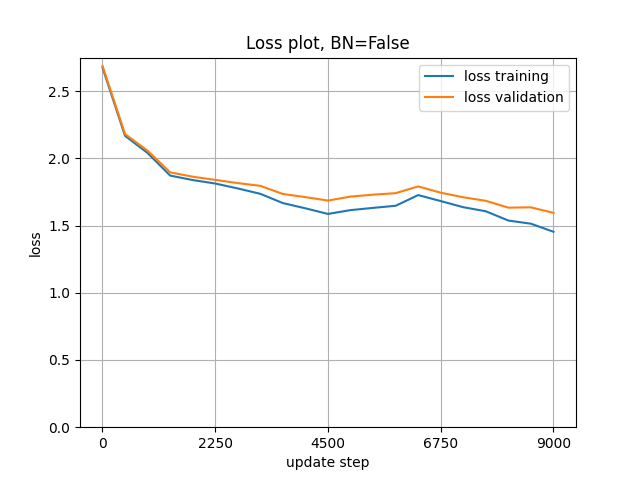
\includegraphics[width=\textwidth]{results/2-2250-9-loss-False.png}
    \end{subfigure}
    \hfill
    \begin{subfigure}{0.45\textwidth}
        \centering
        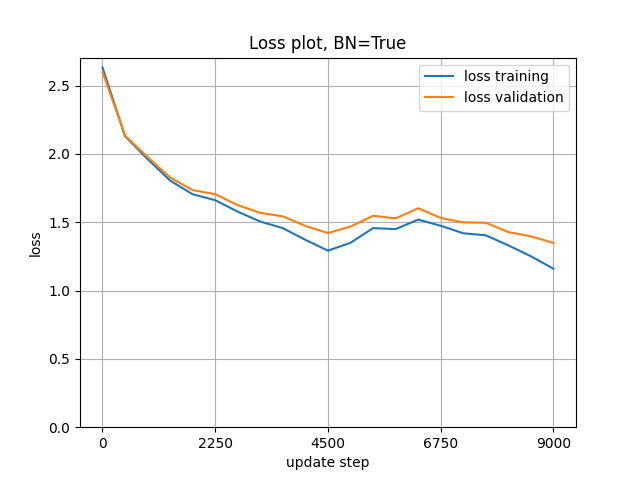
\includegraphics[width=\textwidth]{results/2-2250-9-loss-True.png}
    \end{subfigure}
    \caption{Loss plots for 9-layer networks}
    \label{fig:9-layer}
\end{figure}

\section{Search for lambda}
The search was a coarse search with a wide possible range of lambda. 8 random lambda values where chosen in the $\log_{10}$ range from $-1$ to $-5$. Other parameter settings were cycles$=2$, batch size$\ =100,\ n_s=2250,\ \eta_{min}=10^{-5},\ \eta_{max}=10^{-1}$. The three best performing lambdas were:
\begin{itemize}
    \item Accuracy 0.5174 lambda 0.003933267138576786 log lambda -2.4052465562930467
    \item Accuracy 0.5068 lambda 0.010751078961286456 log lambda -1.968547948453605
    \item Accuracy 0.5052 lambda 7.889600922457556e-05 log lambda -4.102944964034926
\end{itemize}

The best lambda was then used for a finer search. Now 20 values were generated in the log range from $-2.405\pm 1$. The other hyperparameters were the same as in the coarse search. The three best performing lambdas were:

\begin{itemize}
    \item Accuracy 0.5236 lambda 0.013089805517608464 log lambda -1.8830668059516829
    \item Accuracy 0.5234 lambda 0.0087248837545424 log lambda -2.0592403506263293
    \item Accuracy 0.5186 lambda 0.010736512208547537 log lambda -1.9691367777228215
\end{itemize}

Lastly, the best lambda $=0.0131$ was used to train the model. When testing the model on the test data an accuracy of $53.26\%$ was achieved. A plot of the loss function can be seen in \autoref{fig:lossSearch} and all the lambdas and their respective accuracy can be seen in \autoref{search}.

\begin{figure}[H]
    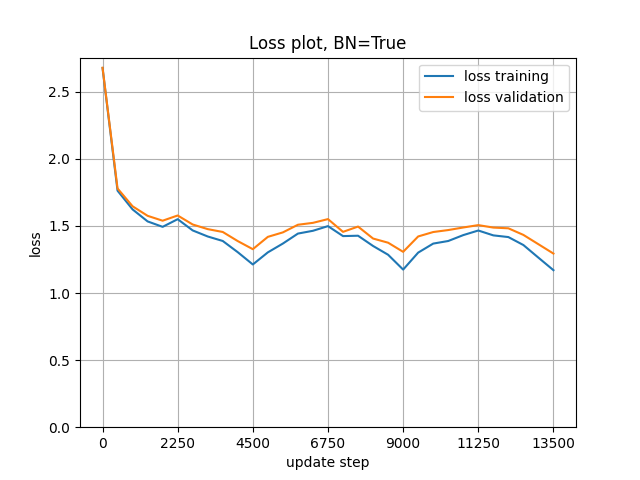
\includegraphics{results/3-2250-3-loss-True.png}
    \caption{Plot of the loss function for the training and validation set with the best lambda.}
    \label{fig:lossSearch}
\end{figure}

\section{Sensitivity to initialization}
Normally, the weights at each layer are initialized proportional to the number of nodes in that layer. To see how stable batch normalization actually is, it was tested to initialize every layer with the same constant variance. When training the model with batch normalization, the initialization does not really seem to be that important; all accuracies are in the same magnitude. However, the same is not true for the case without batch normalization. Here the accuracy is drastically worsen when the variance gets smaller. When $\sigma=1e-4$ the accuracy is just $10\%$ which probably means that the model is trivial and classifies all pictures with the same label.

\begin{table}[H]
    \begin{tabular}{l|ll}
        $\sigma$ & Without batch normalization & With batch normalization \\ \hline
        1e-1     & 53.02\%                     & 53.53\%                  \\
        1e-3     & 39.32\%                     & 53.20\%                  \\
        1e-4     & 10.00\%                     & 53.38\%
    \end{tabular}
\end{table}
\begin{figure}[H]
    \centering
    \begin{subfigure}{0.45\textwidth}
        \centering
        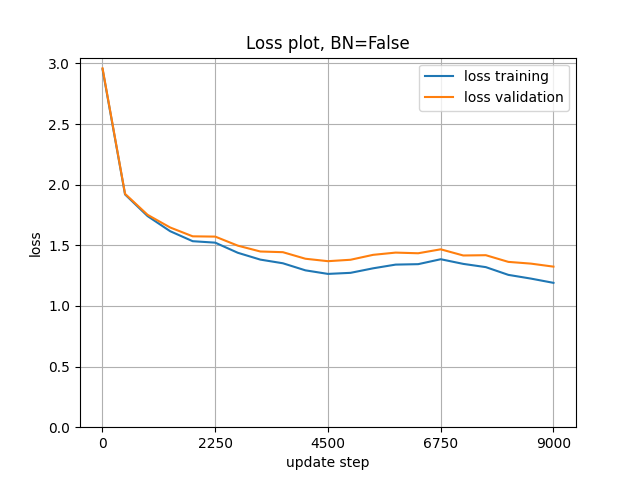
\includegraphics[width=\textwidth]{results/2-2250-3-loss-False-0.1.png}
    \end{subfigure}
    \hfill
    \begin{subfigure}{0.45\textwidth}
        \centering
        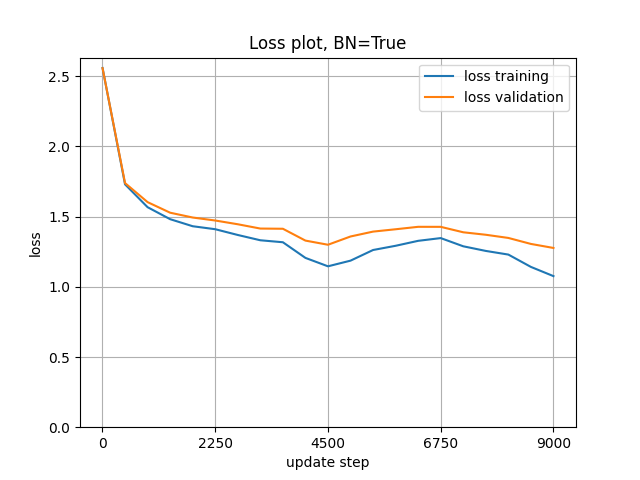
\includegraphics[width=\textwidth]{results/2-2250-3-loss-True-0.1.png}
    \end{subfigure}
    \caption{Loss plots for 3-layer networks with $\sigma=1e-1$}
\end{figure}
\begin{figure}[H]
    \centering
    \begin{subfigure}{0.45\textwidth}
        \centering
        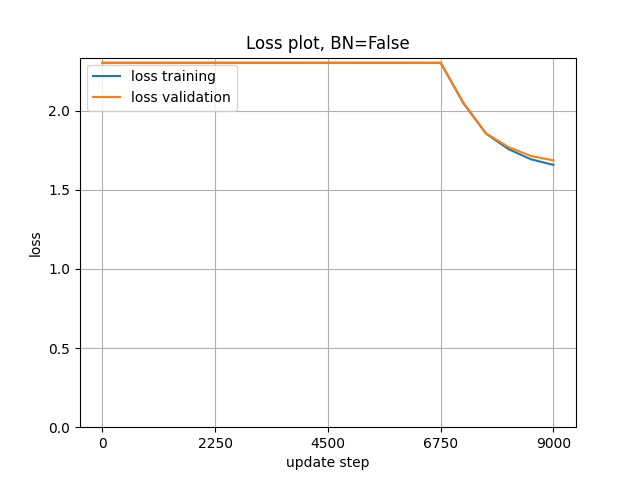
\includegraphics[width=\textwidth]{results/2-2250-3-loss-False-0.001.png}
    \end{subfigure}
    \hfill
    \begin{subfigure}{0.45\textwidth}
        \centering
        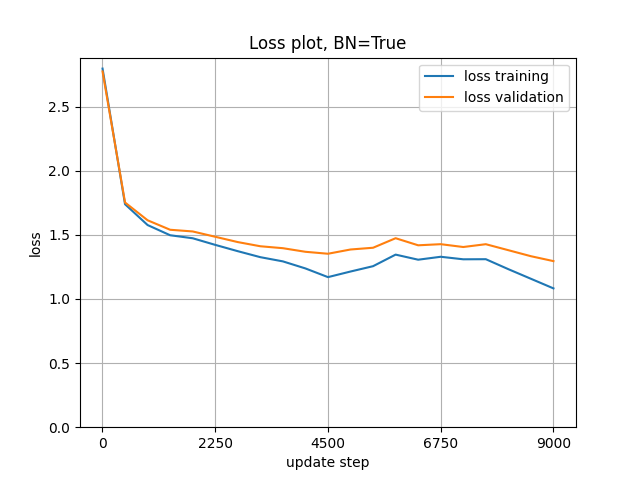
\includegraphics[width=\textwidth]{results/2-2250-3-loss-True-0.001.png}
    \end{subfigure}
    \caption{Loss plots for 3-layer networks with $\sigma=1e-3$}
\end{figure}
\begin{figure}[H]
    \centering
    \begin{subfigure}{0.45\textwidth}
        \centering
        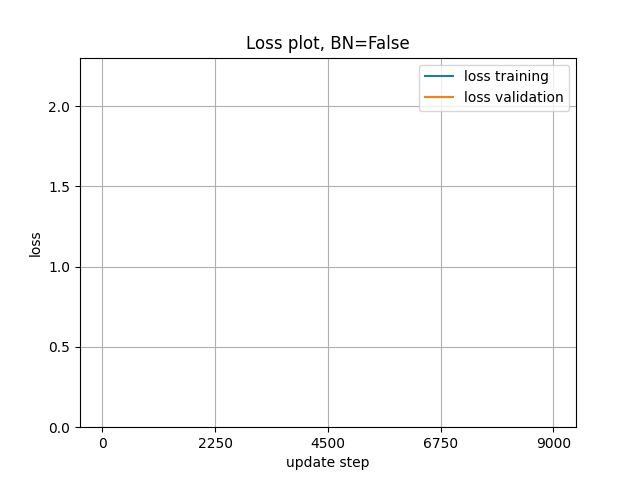
\includegraphics[width=\textwidth]{results/2-2250-3-loss-False-0.0001.png}
    \end{subfigure}
    \hfill
    \begin{subfigure}{0.45\textwidth}
        \centering
        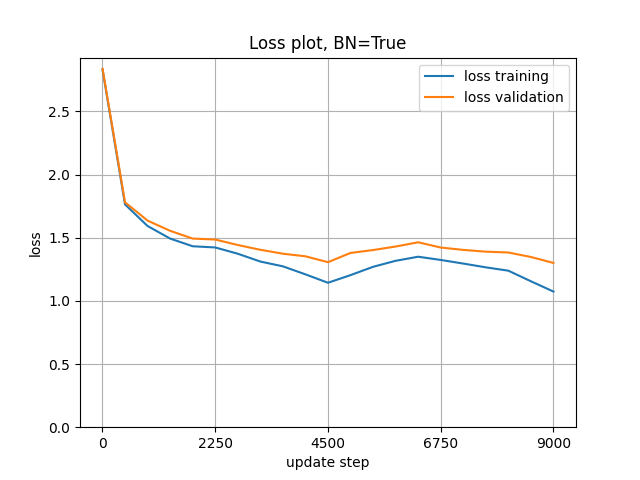
\includegraphics[width=\textwidth]{results/2-2250-3-loss-True-0.0001.png}
    \end{subfigure}
    \caption{Loss plots for 3-layer networks with $\sigma=1e-4$}
\end{figure}

\appendix
\section{Gradients}
\label{gradientData}
\subsection{Without batch normalization}
\VerbatimInput{gradient_error}
\subsection{With batch normalization}
\VerbatimInput{gradient_batch_norm.txt}

\section{Lambda Random Search}
\label{search}
\VerbatimInput{lambda_search3.txt}

\end{document}

